% Provenance (never printed): NSI premiere "Algorithmique: algorithme des k plus proches voisins". See
% sources/book2/BRIEFS.md.
\chapter{Classifying by Neighbours: the k-NN Algorithm}\label{ch:g11:k-nearest-neighbours}

The town's sorting office receives every item posted in the town, and each must go to the right belt: letters to one,
packets to another, parcels to a third. A machine measures each item, its thickness in millimetres and its mass in
grams, but nobody has written down a rule turning these two numbers into a belt. What the office does have is a pile of
items already sorted by hand.

\begin{omfigure}
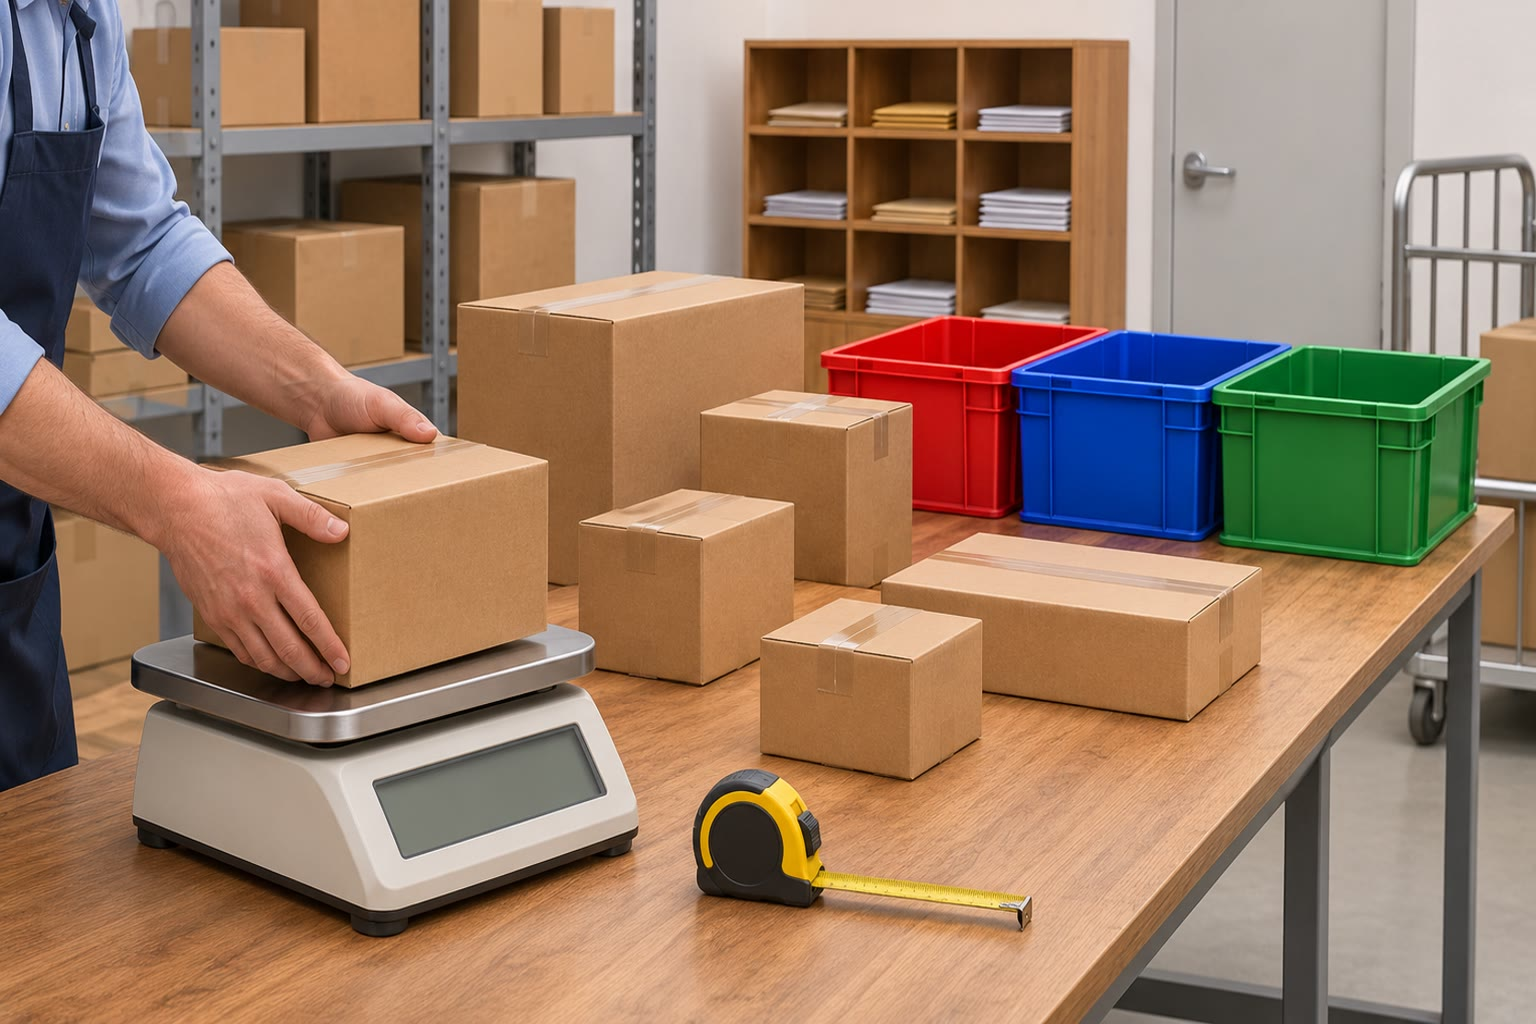
\includegraphics[width=0.55\linewidth]{images/book2/ai/g11-k-nearest-neighbours-parcel-desk.jpg}

{\small Sorting by hand: each item is weighed and measured, then put in the crate of its \omterm{def:g11:k-nearest-neighbours:example}{class}.}
\end{omfigure}

This chapter writes a program that sorts a new item by looking at the items already sorted that resemble it most. The
idea is old and simple, it needs no rule written by hand, and its errors can be measured honestly, provided some items
are kept aside for that purpose.

\begin{recall}
Pseudo-random numbers from a seed, met in the first book of the series, give data that are the same at every run.
\omterm{def:g10:floating-point:float}{Floating-point numbers} are approximations (chapter \ref{ch:g10:floating-point}). \code{sorted(t, key=f)} sorts by a
key (chapter \ref{ch:g10:data-tables}); the cost of an algorithm counts its \omterm{def:g11:cost-of-an-algorithm:elementary}{elementary operations} (chapter
\ref{ch:g11:cost-of-an-algorithm}).
\end{recall}

\section{Learning from labelled examples}\label{sec:g11:k-nearest-neighbours:examples}

\begin{definition}[Labelled example, feature, class]\label{def:g11:k-nearest-neighbours:example}
A \emph{labelled example}\index{labelled example} is an item described by numbers, its
\emph{features}\index{feature}, together with the answer known for it, its \emph{class}\index{class (label)}, also
called its label.
\end{definition}

Here an item is a tuple \code{(thickness, mass, label)}, for instance \code{(13.7, 541, "packet")}. The items of the
office are invented: \code{parcels.py} draws them from a seeded generator, with three classes that overlap, as real
items do: a thick letter weighs as much as a thin packet.

\omcode{code/grade-11/08-k-nearest-neighbours/listings/parcels.py}{1}{24}{The invented items: a seeded generator, and a
split into three parts.}\label{lst:g11:k-nearest-neighbours:parcels}

\begin{definition}[Training set, test set]\label{def:g11:k-nearest-neighbours:training-set}
The \emph{training set}\index{training set} is the set of \omterm{def:g11:k-nearest-neighbours:example}{labelled examples} a method learns from. A \emph{test
set}\index{test set} is a set of \omterm{def:g11:k-nearest-neighbours:example}{labelled examples} kept aside, never used for learning, on which the method's answers
are compared with the known classes.
\end{definition}

The office keeps $180$ items to learn from, $60$ to make choices with, and $60$ that nobody looks at until the very
end.

\omcode{code/grade-11/08-k-nearest-neighbours/listings/show_data.py}{1}{11}{A first look at the
items.}\label{lst:g11:k-nearest-neighbours:show}

\omoutput{code/grade-11/08-k-nearest-neighbours/outputs/show_data.txt}{Three hundred items, three classes, five shown,
and the split.}\label{out:g11:k-nearest-neighbours:show}

\begin{omfigure}
\begin{tikzpicture}
  \begin{axis}[width=11cm, height=7cm, xlabel={thickness (mm)}, ylabel={mass (g)}, xmin=0, xmax=88, ymin=0,
      ymax=1300, scaled y ticks=false, legend pos=north west, legend cell align=left, font=\footnotesize]
    \addplot[only marks, scatter, scatter src=explicit symbolic,
      scatter/classes={letter={mark=o, omDef}, packet={mark=square*, omMeth, mark size=1.6pt},
        parcel={mark=triangle*, omThm, mark size=2.2pt}}]
      table[x=thickness, y=mass, meta=label]{code/grade-11/08-k-nearest-neighbours/figures/parcels_plot.dat};
    \legend{letter, packet, parcel}
  \end{axis}
\end{tikzpicture}

{\small The $180$ items of the \omterm{def:g11:k-nearest-neighbours:training-set}{training set}. Letters sit near the corner; packets and parcels overlap over a wide
band.}
\end{omfigure}

\section{A distance between examples}\label{sec:g11:k-nearest-neighbours:distance}

``Resemble'' needs a number. Two items are drawn as two points, one \omterm{def:g11:k-nearest-neighbours:example}{feature} on each axis, and the distance between them
is the length of the segment joining them, as the mathematics book computes it by Pythagoras' theorem.

\omcode{code/grade-11/08-k-nearest-neighbours/listings/distance.py}{1}{12}{The Euclidean distance between two
items.}\label{lst:g11:k-nearest-neighbours:distance}

\omoutput{code/grade-11/08-k-nearest-neighbours/outputs/distance.txt}{The packet looks closer to the parcel than to
the letter.}\label{out:g11:k-nearest-neighbours:distance}

The output hides a trap. The packet and the parcel differ by $25$~mm, the letter and the packet by $17$~mm; yet the
distances say the opposite of what the eye sees on the thicknesses, because they are almost only differences of mass:
$250$~g counts as $250$, a millimetre counts as $1$. The unit chosen for each \omterm{def:g11:k-nearest-neighbours:example}{feature} decides how much it weighs.

\begin{definition}[Scaling]\label{def:g11:k-nearest-neighbours:scaling}
\emph{Scaling}\index{scaling} the \omterm{def:g11:k-nearest-neighbours:example}{features} means changing each one by the same rule for every item so that all of them
cover comparable ranges. Min-max scaling replaces a value $v$ of a \omterm{def:g11:k-nearest-neighbours:example}{feature} by $(v - \mathit{lo}) / (\mathit{hi} -
\mathit{lo})$, where $\mathit{lo}$ and $\mathit{hi}$ are the smallest and largest values of that \omterm{def:g11:k-nearest-neighbours:example}{feature} in the
\omterm{def:g11:k-nearest-neighbours:training-set}{training set}; the results lie between $0$ and $1$ on the \omterm{def:g11:k-nearest-neighbours:training-set}{training set}.
\end{definition}

\omcode{code/grade-11/08-k-nearest-neighbours/listings/scale.py}{1}{25}{Min-max \omterm{def:g11:k-nearest-neighbours:scaling}{scaling}, computed on the \omterm{def:g11:k-nearest-neighbours:training-set}{training set},
and the new neighbours.}\label{lst:g11:k-nearest-neighbours:scale}

\omoutput{code/grade-11/08-k-nearest-neighbours/outputs/scale.txt}{After \omterm{def:g11:k-nearest-neighbours:scaling}{scaling}, the seven nearest items to
$12$~mm, $150$~g.}\label{out:g11:k-nearest-neighbours:scale}

The bounds come from the \omterm{def:g11:k-nearest-neighbours:training-set}{training set} only: an item kept aside must not change the rule applied to it, or the test
would no longer be a test. Scaled values are \omterm{def:g10:floating-point:float}{floating-point numbers}; two distances that should be equal may differ in
the last digits, which is one more reason to break ties by a fixed rule.

\section{The k nearest neighbours vote}\label{sec:g11:k-nearest-neighbours:vote}

\begin{method}[The k nearest neighbours]\label{met:g11:k-nearest-neighbours:knn}
To predict the \omterm{def:g11:k-nearest-neighbours:example}{class} of a new item $x$ from a \omterm{def:g11:k-nearest-neighbours:training-set}{training set}, with a whole number $k \ge 1$:\index{k nearest neighbours}
\begin{enumerate}
  \item compute the distance from $x$ to every example of the \omterm{def:g11:k-nearest-neighbours:training-set}{training set};
  \item keep the $k$ examples with the smallest distances, the $k$ nearest neighbours;
  \item answer the \omterm{def:g11:k-nearest-neighbours:example}{class} that is most common among them; on a tie, a fixed rule decides, here the \omterm{def:g11:k-nearest-neighbours:example}{class} of the
    nearest of the tied ones.
\end{enumerate}
\end{method}

\omcode{code/grade-11/08-k-nearest-neighbours/listings/knn.py}{1}{30}{The vote of the $k$ nearest neighbours, and one
new item.}\label{lst:g11:k-nearest-neighbours:knn}

\omoutput{code/grade-11/08-k-nearest-neighbours/outputs/knn.txt}{Without \omterm{def:g11:k-nearest-neighbours:scaling}{scaling}: the seven nearest to $12$~mm,
$150$~g, and the votes for $k = 1$, $3$, $7$.}\label{out:g11:k-nearest-neighbours:knn}

\begin{omfigure}
\begin{tikzpicture}[x=1cm, y=1cm, font=\footnotesize]
  \foreach \x/\y/\c in {0.6/1.1/0, 1.2/0.3/0, 2.6/2.0/1, 3.1/1.2/1, 2.0/2.7/1, 3.6/2.6/1, 1.1/2.2/0, 4.6/1.5/2,
      4.9/2.8/2, 0.4/2.9/0, 3.9/0.5/2, 5.3/0.9/2, 1.7/-0.1/0} {
    \ifcase\c \draw[omDef, thick] (\x,\y) circle (2.2pt);
    \or \fill[omMeth] (\x-0.07,\y-0.07) rectangle (\x+0.07,\y+0.07);
    \or \fill[omThm] (\x,\y+0.1) -- (\x-0.09,\y-0.06) -- (\x+0.09,\y-0.06) -- cycle; \fi
  }
  \fill (2.4,1.6) circle (2.5pt) node[below left] {$x$};
  \draw[dashed] (2.4,1.6) circle (1.562cm);
  \foreach \x/\y in {2.6/2.0, 3.1/1.2, 2.0/2.7, 1.1/2.2, 3.6/2.6}
    \draw[black!60] (2.4,1.6) -- (\x,\y);
  \node[right, align=left] at (6,2) {$k = 5$: four squares,\\ one circle:\\ square wins};
\end{tikzpicture}

{\small A new item $x$ and its five nearest neighbours, joined to it; the dashed circle passes through the fifth.
Four of the five are squares, so $x$ is given the \omterm{def:g11:k-nearest-neighbours:example}{class} of the squares.}
\end{omfigure}

With $k = 1$ the answer follows the single nearest example, however unusual it is; a larger $k$ smooths the answer by
asking more examples. The two pictures below colour every point of the plane by the \omterm{def:g11:k-nearest-neighbours:example}{class} the method would give it.

\begin{omfigure}
\begin{tikzpicture}
  \foreach \k/\xs in {1/0, 7/7.2} {
  \begin{axis}[at={(\xs cm,0)}, width=7cm, height=6cm, xmin=-1, xmax=81, ymin=-15, ymax=1215,
      scaled y ticks=false, title={$k = \k$}, xlabel={thickness (mm)}, ylabel={mass (g)}, font=\scriptsize]
    \addplot[only marks, scatter, scatter src=explicit symbolic, mark=square*, mark size=2.2pt,
      scatter/classes={letter={omDef!35}, packet={omMeth!30}, parcel={omThm!30}}]
      table[x=thickness, y=mass, meta=label]{code/grade-11/08-k-nearest-neighbours/figures/regions_k\k.dat};
  \end{axis}
  }
\end{tikzpicture}

{\small The \omterm{def:g11:k-nearest-neighbours:example}{class} predicted at each point of a grid, with scaled \omterm{def:g11:k-nearest-neighbours:example}{features}: blue for letter, green for packet, red for
parcel. With $k = 1$ the frontier between packet and parcel is ragged and leaves islands; with $k = 7$ it is
smoother.}
\end{omfigure}

\section{Measuring the error}\label{sec:g11:k-nearest-neighbours:error}

\begin{definition}[Error rate]\label{def:g11:k-nearest-neighbours:error-rate}
The \emph{error rate}\index{error rate} of a method on a set of \omterm{def:g11:k-nearest-neighbours:example}{labelled examples} is the number of examples whose
predicted \omterm{def:g11:k-nearest-neighbours:example}{class} differs from the known \omterm{def:g11:k-nearest-neighbours:example}{class}, divided by the number of examples.
\end{definition}

On which examples? On the \omterm{def:g11:k-nearest-neighbours:training-set}{training set} itself, $k = 1$ never errs: each example's nearest neighbour is itself, at
distance $0$. That says nothing about new items. The error must be measured on examples the method has not seen.

\omcode{code/grade-11/08-k-nearest-neighbours/listings/error_rate.py}{1}{26}{The \omterm{def:g11:k-nearest-neighbours:error-rate}{error rate} for each $k$, on the
\omterm{def:g11:k-nearest-neighbours:training-set}{training set} and on the validation set.}\label{lst:g11:k-nearest-neighbours:error-rate}

\omoutput{code/grade-11/08-k-nearest-neighbours/outputs/error_rate.txt}{The training error is $0$ for $k = 1$ and $2$;
the validation error tells more.}\label{out:g11:k-nearest-neighbours:error-rate}

Choosing $k$ is itself a kind of learning: the $60$ validation items serve to choose, and the $60$ test items, never
used for any choice, give the honest final error. If $k$ were chosen on the test items, their error would flatter
the method.

\omcode{code/grade-11/08-k-nearest-neighbours/listings/choose_k.py}{1}{9}{The smallest $k$ with the fewest validation
errors.}\label{lst:g11:k-nearest-neighbours:choose}

\omoutput{code/grade-11/08-k-nearest-neighbours/outputs/choose_k.txt}{Five values of $k$ tie; the smallest is
chosen.}\label{out:g11:k-nearest-neighbours:choose}

\begin{omfigure}
\begin{tikzpicture}
  \begin{axis}[width=10cm, height=6cm, xlabel={$k$}, ylabel={validation error (\%)}, xmin=0.5, xmax=15.5, ymin=0,
      ymax=25, xtick={1,3,...,15}, legend pos=north west, legend cell align=left, font=\footnotesize]
    \addplot[omThm, thick, dashed, mark=o] table[x=k, y=unscaled]
      {code/grade-11/08-k-nearest-neighbours/figures/error_vs_k.dat};
    \addplot[omDef, thick, mark=*] table[x=k, y=scaled]
      {code/grade-11/08-k-nearest-neighbours/figures/error_vs_k.dat};
    \legend{unscaled, scaled}
  \end{axis}
\end{tikzpicture}

{\small The validation error against $k$. \omterm{def:g11:k-nearest-neighbours:scaling}{Scaling} lowers it for every $k$: with scaled \omterm{def:g11:k-nearest-neighbours:example}{features} it stays between $5$ and
$10\,\%$, while without \omterm{def:g11:k-nearest-neighbours:scaling}{scaling} it climbs towards $20\,\%$ as $k$ grows.}
\end{omfigure}

\section{What the method cannot do, and its cost}\label{sec:g11:k-nearest-neighbours:cost}

The method learns nothing in advance: it keeps the whole \omterm{def:g11:k-nearest-neighbours:training-set}{training set} and does all its work at each prediction. With
$n$ examples, each prediction computes $n$ distances, then sorts them.

\omcode{code/grade-11/08-k-nearest-neighbours/listings/knn_cost.py}{1}{21}{Counting the distances
computed.}\label{lst:g11:k-nearest-neighbours:cost}

\omoutput{code/grade-11/08-k-nearest-neighbours/outputs/knn_cost.txt}{$180$ distances per prediction, whatever
$k$.}\label{out:g11:k-nearest-neighbours:cost}

For $m$ predictions, $m \times n$ distances, each taking a few operations per \omterm{def:g11:k-nearest-neighbours:example}{feature}: a cost that grows like
$m \times n \times d$ with $d$ \omterm{def:g11:k-nearest-neighbours:example}{features}, plus the sorts. A post office handling a million items a day with a million
examples would compute $10^{12}$ distances a day. Faster methods exist that organise the examples in advance, or
learn a compact rule instead of keeping them all.

\begin{remark}
With many \omterm{def:g11:k-nearest-neighbours:example}{features}, a further difficulty appears: in a space of many dimensions, almost all points are far from one
another, and the nearest neighbour is hardly nearer than the others. The vote then means little. The series' books on
artificial intelligence take up these questions, and the methods that answer them.
\end{remark}

\begin{history}[Neighbours]
% ledger: g11:fix-hodges
% ledger: g11:cover-hart-1967
The nearest-neighbour rule was described by the statisticians E. Fix and J. L. Hodges in a report long kept unpublished,
finally printed in a statistics journal in 1989. In January 1967, T. Cover and P. Hart published an article proving
that, with enough examples, the error of the rule with $k = 1$ is at most twice the smallest error any rule could
reach.
\end{history}

\section{Exercises}\label{sec:g11:k-nearest-neighbours:exercises}

\begin{exercise}[$\star$]\label{exo:g11:k-nearest-neighbours:1}
Compute the distance between the items $(2~\text{mm}, 30~\text{g})$ and $(5~\text{mm}, 34~\text{g})$, without
\omterm{def:g11:k-nearest-neighbours:scaling}{scaling}.
\end{exercise}

\begin{exercise}[$\star$]\label{exo:g11:k-nearest-neighbours:2}
A tiny \omterm{def:g11:k-nearest-neighbours:training-set}{training set}: A at $(1, 1)$, A at $(2, 1)$, B at $(4, 3)$, B at $(5, 4)$, A at $(3, 2)$. Which \omterm{def:g11:k-nearest-neighbours:example}{class} does the
method predict for $(4, 4)$ with $k = 3$?
\end{exercise}

\begin{exercise}[$\star$]\label{exo:g11:k-nearest-neighbours:3}
With the same \omterm{def:g11:k-nearest-neighbours:training-set}{training set}, list the five examples from the nearest to the farthest from $(3.5, 3)$.
\end{exercise}

\begin{exercise}[$\star$]\label{exo:g11:k-nearest-neighbours:4}
A confusion table counts, for each true \omterm{def:g11:k-nearest-neighbours:example}{class} (row), the predicted classes (columns). Compute the \omterm{def:g11:k-nearest-neighbours:error-rate}{error rate}.
\begin{center}
\begin{tabular}{lrrr}
  true \textbackslash{} predicted & letter & packet & parcel \\ \hline
  letter & $25$ & $1$ & $0$ \\
  packet & $1$ & $17$ & $1$ \\
  parcel & $0$ & $1$ & $14$
\end{tabular}
\end{center}
\end{exercise}

\begin{exercise}[$\star$]\label{exo:g11:k-nearest-neighbours:5}
Write \code{distance(a, b)} for items with any number of \omterm{def:g11:k-nearest-neighbours:example}{features}, the label being the last element of each tuple.
\end{exercise}

\begin{exercise}[$\star\star$]\label{exo:g11:k-nearest-neighbours:6}
To estimate the error without a validation set, a student predicts each item of the \omterm{def:g11:k-nearest-neighbours:training-set}{training set} with
\code{knn_predict(items, x, 1)}, and finds an error of $0$ for every data set. Find the fault and correct it.
\end{exercise}

\begin{exercise}[$\star\star$]\label{exo:g11:k-nearest-neighbours:7}
Write \code{knn_predict(train, x, k)}, with ties broken by the \omterm{def:g11:k-nearest-neighbours:example}{class} of the nearest of the tied ones.
\end{exercise}

\begin{exercise}[$\star\star$]\label{exo:g11:k-nearest-neighbours:8}
In the \omterm{def:g11:k-nearest-neighbours:training-set}{training set}, thickness runs from $0.5$ to $84.7$~mm and mass from $5$ to $1231$~g. Compute, with and without
\omterm{def:g11:k-nearest-neighbours:scaling}{scaling}, the distances from the new item $(12, 150)$ to $(5.3, 159)$ and to $(13.9, 133)$. Which is nearer in each
case?
\end{exercise}

\begin{exercise}[$\star\star$]\label{exo:g11:k-nearest-neighbours:9}
A vote is written \code{max(set(labels), key=labels.count)}, where \code{labels} is the list of the $k$ neighbours'
classes. On some items the program answers differently from one run to the next. Why?
\end{exercise}

\begin{exercise}[$\star\star$]\label{exo:g11:k-nearest-neighbours:10}
In the output of \code{error_rate.py}, the training error is $0$ for $k = 1$. Explain why. Can it be different from
$0$ for some data?
\end{exercise}

\begin{exercise}[$\star\star$]\label{exo:g11:k-nearest-neighbours:11}
Write \code{minmax(train)}, which returns a function \omterm{def:g11:k-nearest-neighbours:scaling}{scaling} an item with bounds taken from \code{train}, for any
number of \omterm{def:g11:k-nearest-neighbours:example}{features}.
\end{exercise}

\begin{exercise}[$\star\star\star$]\label{exo:g11:k-nearest-neighbours:12}
Give the cost of predicting $m$ items with $n$ examples and $d$ \omterm{def:g11:k-nearest-neighbours:example}{features}, counting the operations on \omterm{def:g11:k-nearest-neighbours:example}{features} for the
distances and the comparisons for the sorts. What changes if the $k$ nearest are found by $k$ scans for the smallest
remaining distance instead of a sort?
\end{exercise}

\begin{exercise}[$\star\star\star$]\label{exo:g11:k-nearest-neighbours:13}
Write \code{loo_error(items, k)}, the leave-one-out error: each item is predicted from all the others, and the \omterm{def:g11:k-nearest-neighbours:error-rate}{error
rate} is computed over all the items.
\end{exercise}

\begin{exercise}[$\star\star\star$]\label{exo:g11:k-nearest-neighbours:14}
What does the method predict when $k$ equals the number $n$ of training examples? What \omterm{def:g11:k-nearest-neighbours:error-rate}{error rate} does it then have on
the validation set of the chapter?
\end{exercise}

\begin{exercise}[$\star\star\star$]\label{exo:g11:k-nearest-neighbours:15}
Write \code{weighted_predict(train, x, k)}, in which each of the $k$ neighbours votes with a weight $1/\text{distance}$.
On the scaled validation set it makes $5$ errors with $k = 5$, where the plain vote makes $3$, but $3$ errors for
every $k$ from $6$ to $12$. What do the two votes do differently?
\end{exercise}

\section{Problem: The Sorting Office}\label{sec:g11:k-nearest-neighbours:problem}

\begin{problem}[{Weekend problem --- does k-NN beat a rule of thumb?}]\label{pb:g11:k-nearest-neighbours:1}
The sorting office compares the method with the simplest possible rule, always answering the most common \omterm{def:g11:k-nearest-neighbours:example}{class} of the
\omterm{def:g11:k-nearest-neighbours:training-set}{training set}, then chooses $k$ and the \omterm{def:g11:k-nearest-neighbours:scaling}{scaling} on the validation set, and finally measures the error once, on the \omterm{def:g11:k-nearest-neighbours:training-set}{test
set}.

\omcode{code/grade-11/08-k-nearest-neighbours/listings/sorting_office.py}{1}{22}{The baseline, the choice of $k$ and
the final test.}\label{lst:g11:k-nearest-neighbours:office}

\omoutput{code/grade-11/08-k-nearest-neighbours/outputs/sorting_office.txt}{The baseline, the validation errors with
and without \omterm{def:g11:k-nearest-neighbours:scaling}{scaling}, and the final error.}\label{out:g11:k-nearest-neighbours:office}

\medskip\noindent\textbf{Part I --- The data and a baseline.}
\begin{enumerate}
  \item What are the \omterm{def:g11:k-nearest-neighbours:example}{features}, and what is the \omterm{def:g11:k-nearest-neighbours:example}{class}, of an item?
  \item Why are the items invented and drawn from a seeded generator?
  \item The \omterm{def:g11:k-nearest-neighbours:training-set}{training set} has $84$ packets, $57$ letters and $39$ parcels. Which \omterm{def:g11:k-nearest-neighbours:example}{class} does the baseline always answer?
  \item The validation set has $27$ packets out of $60$. Check the baseline's validation error.
  \item The \omterm{def:g11:k-nearest-neighbours:training-set}{test set} has $19$ packets out of $60$. Check the baseline's test error. Why does it differ from the
    validation error?
\end{enumerate}

\medskip\noindent\textbf{Part II --- k-NN without scaling.}
\begin{enumerate}[resume]
  \item From the unscaled column, what is the smallest validation error, and for which $k$?
  \item How many validation items does a $20\,\%$ error stand for?
  \item Why does the unscaled error grow with $k$? Think of which \omterm{def:g11:k-nearest-neighbours:example}{feature} decides the neighbours.
  \item Is the unscaled method still much better than the baseline?
\end{enumerate}

\medskip\noindent\textbf{Part III --- Scaling.}
\begin{enumerate}[resume]
  \item From the scaled column, which values of $k$ give the smallest validation error?
  \item The program keeps the first $k$ reaching the smallest error. Which $k$ is chosen?
  \item Why are the bounds of the \omterm{def:g11:k-nearest-neighbours:scaling}{scaling} taken from the \omterm{def:g11:k-nearest-neighbours:training-set}{training set} only?
  \item The scaled error for $k = 1$ is $10\,\%$, for $k = 5$ it is $5\,\%$. Explain the difference with the pictures
    of the decision regions.
  \item How many fewer validation errors does \omterm{def:g11:k-nearest-neighbours:scaling}{scaling} make at $k = 5$?
\end{enumerate}

\medskip\noindent\textbf{Part IV --- The final test.}
\begin{enumerate}[resume]
  \item What is the final test error, and how many test items does it stand for?
  \item With \omterm{def:g11:k-nearest-neighbours:scaling}{scaling}, the test errors for $k = 1$ to $15$ are $4, 4, 3, 3, 4, 4, \dots$: $k = 3$ would have done better
    on the \omterm{def:g11:k-nearest-neighbours:training-set}{test set}. Why must the office still keep $k = 5$?
  \item The four test items in error are a parcel of $33.8$~mm and $349$~g, a packet of $0.5$~mm and $152$~g, a
    packet of $10.4$~mm and $5$~g, and a parcel of $20.9$~mm and $573$~g. Why are they hard?
  \item Every prediction computes $180$ distances. How many for a day of $5000$ items?
  \item How could the office reduce the error further, without changing the method?
  \item State the result: the chosen $k$, its test error, and the baseline's test error.
\end{enumerate}
\end{problem}
